\documentclass[conference]{IEEEtran}

% ============================================================================
% PACKAGES
% ============================================================================
\usepackage[utf8]{inputenc}
\usepackage[T1]{fontenc}
\usepackage{graphicx}
\usepackage{booktabs}
\usepackage{array}
\usepackage{amsmath, amssymb}
\usepackage{hyperref}
\usepackage{caption}
\usepackage{subcaption}
\usepackage{float}
\usepackage{xcolor}
\usepackage{cite}
\usepackage{url}
\usepackage{multirow}
\usepackage{tabularx}
\usepackage{balance}
\usepackage{stfloats}

% Fix for IEEEtran + subcaption compatibility
\makeatletter
\let\MYcaption\@makecaption
\makeatother
\usepackage[font=footnotesize]{subcaption}
\makeatletter
\let\@makecaption\MYcaption
\makeatother

% ============================================================================
% TITLE
% ============================================================================
\title{Bangladesh National Election 2026: Big Data Correlation and Predictive Analytics Using Apache Spark}

\author{
    \IEEEauthorblockN{Sunzid Ashraf Mahi}
    \IEEEauthorblockA{ID: 2021-2-60-148\\sunzidashraf@gmail.com\\East West University\\Dhaka, Bangladesh}
    \and
    \IEEEauthorblockN{Md. Sadik Shahriar}
    \IEEEauthorblockA{ID: 2023-2-60-103\\shahriarsadik@gmail.com\\East West University\\Dhaka, Bangladesh}
    \and
    \IEEEauthorblockN{Abdullah Saleh Mahmud}
    \IEEEauthorblockA{ID: 2023-1-60-215\\mahmudsaleh1177@gmail.com\\East West University\\Dhaka, Bangladesh}
}

\begin{document}
\maketitle

% ============================================================================
% ABSTRACT
% ============================================================================
\begin{abstract}
This paper presents a comprehensive big data analytics pipeline for the 13th Bangladesh National Parliamentary Election held on February 12, 2026, conducted concurrently with the July Charter constitutional referendum. Leveraging Apache Spark, Spark SQL, and Spark MLlib on Google Colab, we integrate constituency level election results with granular socio-economic indicators derived from the Bangladesh Bureau of Statistics (BBS) 2022 Population and Housing Census. Our data engineering pipeline processes over 95,000 raw demographic records across four census dimensions and condenses them into 269 ML-ready constituency profiles via a custom geospatial mapping bridge and K-Nearest Neighbors (KNN) imputation. The analytical pipeline encompasses: (i)~Pearson and Spearman dual correlation analysis revealing strong negative associations between internet penetration and voter turnout ($r = -0.5948$); (ii)~regression modeling achieving $R^2 = 0.6302$ for voter turnout prediction; (iii)~Random Forest classification of winning coalitions attaining 76.79\% accuracy with AUC-ROC of 0.7738; and (iv)~K-Means clustering identifying two dominant constituency archetypes (Silhouette = 0.7078). Extended hypothesis testing across 13 socio-political hypotheses reveals a U-shaped wealth radicalism relationship, statistically significant coalition--referendum cleavages ($p = 0.000781$), and a border radicalization effect (OR = 1.90). Youth demographics emerge as the primary structural determinant of electoral outcomes.
\end{abstract}

\begin{IEEEkeywords}
Big Data Analytics, Apache Spark, MLlib, Bangladesh Election 2026, Random Forest, K-Means Clustering, Electoral Prediction, Socio-Economic Analysis
\end{IEEEkeywords}

% ============================================================================
% I. INTRODUCTION
% ============================================================================
\section{Introduction}

The 13th Bangladesh National Parliamentary Election, held on February~12, 2026, featured a concurrent constitutional referendum on the ``July Charter.'' The election was dominated by two coalition blocs: the \textbf{BNP Coalition} (212 seats) and the \textbf{Jamaat/Reform Coalition} (77 seats), with 8~seats captured by independents.

Despite the availability of granular census data, no systematic big data analysis has quantified the relationship between socio-economic indicators and electoral outcomes. This project addresses four research questions: (RQ1)~What are the statistically significant correlations between socio-economic indicators and electoral outcomes? (RQ2)~Can regression models predict voter turnout from census data? (RQ3)~Can a classifier predict the winning coalition from demographics alone? (RQ4)~Do constituencies cluster into distinct socio-economic archetypes with divergent voting patterns?

We implement a complete end-to-end pipeline using Apache Spark (PySpark) on Google Colab, spanning data ingestion, geospatial mapping, feature engineering, imputation, correlation analysis, regression, classification, clustering, and extended hypothesis testing.

% ============================================================================
% II. DATA SOURCES AND ENGINEERING
% ============================================================================
\section{Data Sources and Engineering}

\subsection{Data Sources}
The project integrates two primary data families:

\textbf{BBS Census 2022:} Four thematic sheets were extracted---SDG Tracking (Internet, Clean Fuel, Sanitation, Financial Inclusion), Age-Structure Demographics (Youth/Senior Electorate, First-Time Voters, NEET Youth), Gender Demographics (Female Population), and Housing Structure (Pucca/Brick housing, Extreme Poverty proxy).

\textbf{Election Commission Results:} Constituency-level results for all 300 seats, including candidate vote counts, party mappings, and July Charter referendum YES/NO percentages (available for 168 constituencies).

\textbf{Constituency Boundaries:} A PDF listing 300 parliamentary boundaries was parsed using \texttt{pdfplumber} for the geospatial bridge.

\subsection{Data Engineering Pipeline}

The pipeline transforms over 95,000 raw census records into 269 ML-ready constituency profiles through seven stages:

\textbf{Stages 1--2: Ingestion and Feature Extraction.} BBS Excel files were loaded via \texttt{pd.read\_excel()} with schema sanitization. Four feature families were extracted: SDG indicators, youth/age demographics (with Voting Age Population correction excluding ages 0--14), gender ratios, and housing/wealth metrics. The Wealth Polarization Index was computed as $\text{WPI\_Log} = \log(\text{Extreme\_Poverty} / \text{Pucca})$.

\textbf{Stage 3: Grand Merge.} Feature families were fused using a LEFT JOIN to preserve 44 constituencies with missing SDG data.

\textbf{Stages 4--5: Geospatial Bridge.} The BBS administrative hierarchy (Districts/Upazilas/Thanas) was mapped to EC constituency numbers via: (i)~NLP fuzzy matching of location names against boundary descriptions, (ii)~hardcoded city thana-to-constituency maps for Dhaka, Chattogram, Khulna, and (iii)~district alias dictionaries for spelling discrepancies. Coverage achieved: \textbf{269 of 300 constituencies (89.6\%)}.

\textbf{Stage 6: KNN Imputation.} Twelve districts (75 seats) lacked SDG sheets. \texttt{KNNImputer} ($k=5$, distance-weighted) estimated missing values from the 5 most demographically similar constituencies, preserving multivariate correlation structure.

\textbf{Stage 7: Election Results Cleaning.} Vote count strings were parsed, a known anomaly corrected, party names translated via reference CSV, and fringe candidates removed.

\subsection{Feature Engineering}

Table~\ref{tab:features} summarizes the 18 features used in the ML pipeline.

\begin{table}[t]
\centering
\caption{Engineered Feature Set}
\label{tab:features}
\footnotesize
\begin{tabular}{l l}
\toprule
\textbf{Feature} & \textbf{Source / Description} \\
\midrule
Youth\_Electorate\_Pct & BBS C-05: Electorate aged 18--35 \\
Senior\_Electorate\_Pct & BBS C-05: Electorate aged 60+ \\
First\_Time\_Voter\_Pct & BBS C-05: Electorate aged 18--22 \\
NEET\_Youth\_Pct & BBS C-05: Youth not in edu/work \\
Female\_Pop\_Pct & BBS Gender: Female share \\
Pucca\_Pct & BBS C-14: Brick housing (wealth) \\
Extreme\_Poverty\_Pct & BBS C-14: Jhupri+Kancha housing \\
WPI\_Log & Engineered: log(Poverty/Pucca) \\
Internet\_Pct & BBS SDG: Internet access \\
Clean\_Fuel\_Pct & BBS SDG: Clean cooking fuel \\
Sanitation\_Pct & BBS SDG: Sanitation access \\
Organized\_Learning\_Pct & BBS SDG: Education participation \\
Financial\_Inclusion\_Pct & BBS SDG: Financial services \\
Urban\_Proxy & Engineered: Urbanization index \\
Digital\_Youth\_Index & Engineered: Internet$\times$Youth \\
Infrastructure\_Comp. & Engineered: Sanitation+Fuel \\
Deprivation\_Index & Engineered: Poverty+NEET \\
Cluster\_ID & K-Means: Constituency archetype \\
\bottomrule
\end{tabular}
\end{table}

% ============================================================================
% III. SYSTEM ARCHITECTURE
% ============================================================================
\section{System Architecture}

The pipeline was executed on Google Colab using PySpark for distributed processing, Spark SQL for structured queries, and Spark MLlib for all machine learning tasks (\texttt{Correlation}, \texttt{LinearRegression}, \texttt{RandomForestClassifier}, \texttt{RandomForestRegressor}, \texttt{KMeans}, \texttt{StandardScaler}, \texttt{VectorAssembler}, \texttt{StringIndexer}). scikit-learn was used exclusively for \texttt{KNNImputer}. Visualizations were generated with Matplotlib and Seaborn via Pandas conversion.

% ============================================================================
% IV. EXPLORATORY DATA ANALYSIS
% ============================================================================
\section{Exploratory Data Analysis}

EDA was performed on the enriched dataset (\texttt{grand\_df\_enriched}) to understand distributional properties. Fig.~\ref{fig:eda} presents the target variable distributions, feature distributions, and full correlation matrix.

\begin{figure*}[t]
\centering
\begin{subfigure}[b]{0.32\textwidth}
    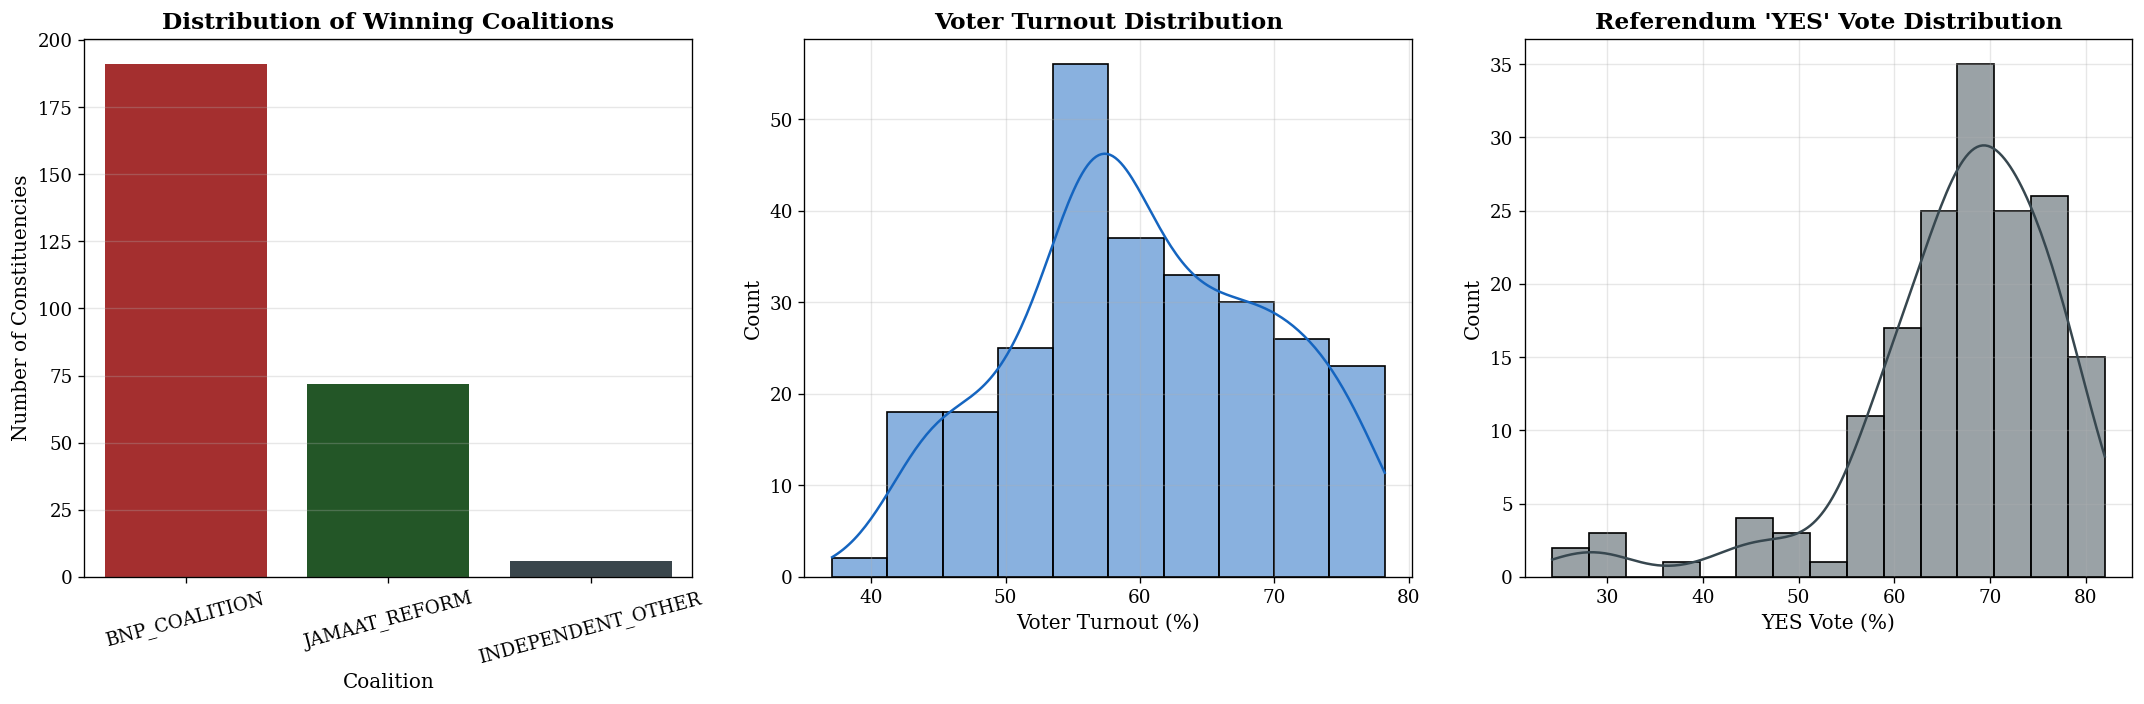
\includegraphics[width=\textwidth]{exported_plots/EDA_2_Target_Variable_Distributions.png}
    \caption{Target distributions}
\end{subfigure}
\hfill
\begin{subfigure}[b]{0.32\textwidth}
    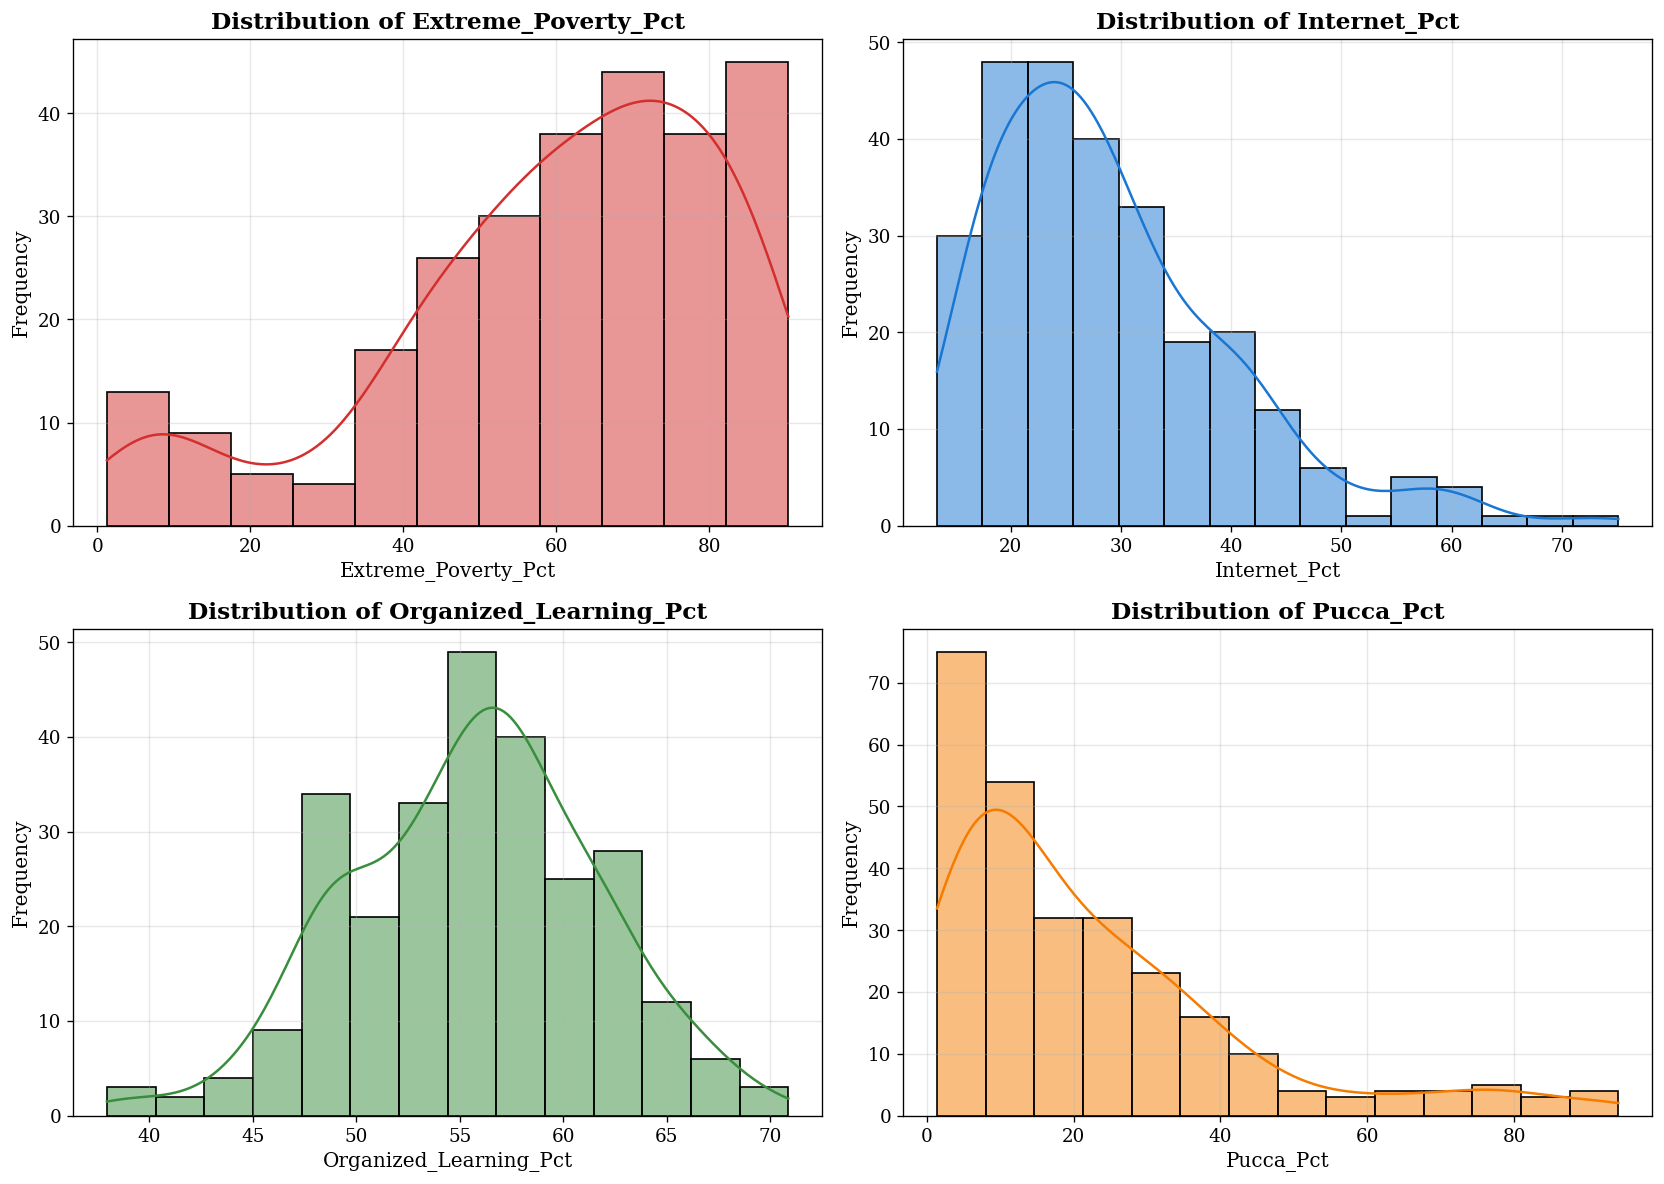
\includegraphics[width=\textwidth]{exported_plots/EDA_3_Socio_Economic_Feature_Distributions_Univariate_Analysis.png}
    \caption{Feature distributions}
\end{subfigure}
\hfill
\begin{subfigure}[b]{0.32\textwidth}
    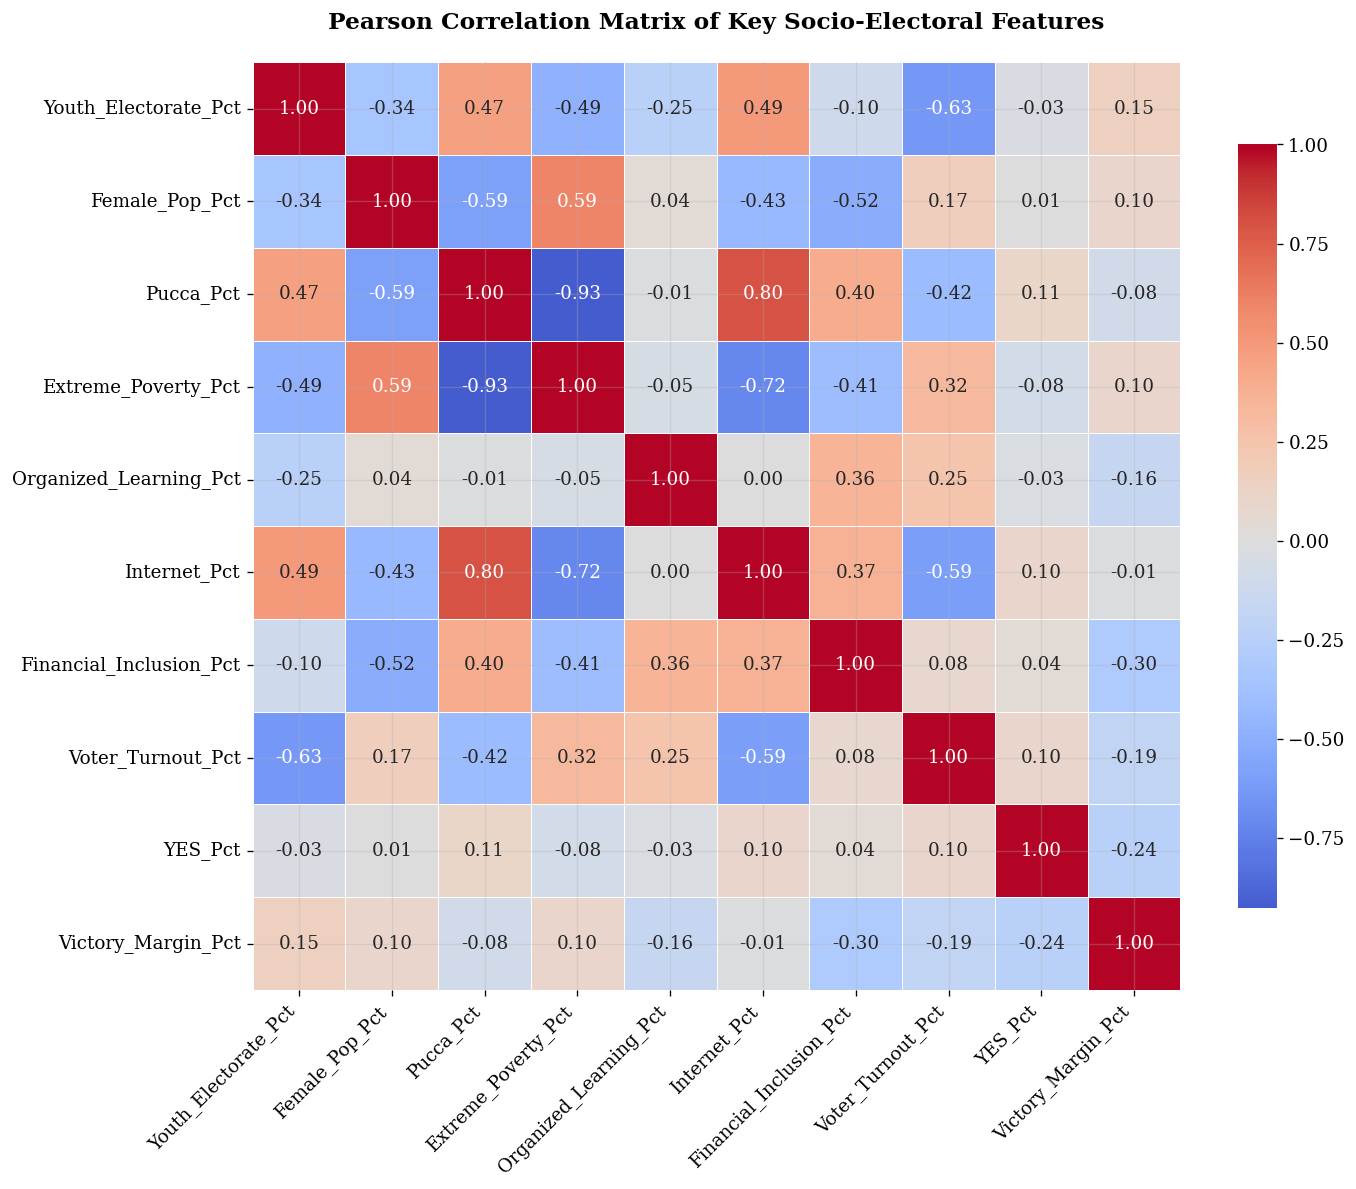
\includegraphics[width=\textwidth]{exported_plots/EDA_4_Correlation_Analysis_Bivariate_Analysis.png}
    \caption{Correlation matrix}
\end{subfigure}
\caption{Exploratory Data Analysis: (a) Coalition victory and turnout distributions, (b) univariate socio-economic feature distributions, (c) Pearson correlation matrix across 269 constituencies.}
\label{fig:eda}
\end{figure*}

% ============================================================================
% V. CORRELATION ANALYSIS
% ============================================================================
\section{Correlation Analysis}

Pearson and Spearman correlation matrices were computed using \texttt{pyspark.ml.stat.Correlation} on $N = 268$ constituencies. Table~\ref{tab:corr} presents hypothesis-driven results.

\begin{table}[t]
\centering
\caption{Key Correlation Results}
\label{tab:corr}
\footnotesize
\begin{tabular}{l r r l}
\toprule
\textbf{Variables} & \textbf{Pearson} & \textbf{Spearman} & \textbf{Result} \\
\midrule
Internet vs.\ Turnout & $-0.5948$ & $-0.5392$ & \textbf{Confirmed} \\
Wealth Pol.\ vs.\ Margin & $+0.0405$ & $+0.0109$ & Rejected \\
NEET vs.\ Turnout & $+0.2460$ & $+0.0720$ & Rejected \\
Poverty vs.\ Turnout & $+0.3228$ & $+0.1857$ & Moderate \\
Urban vs.\ Turnout & $-0.5111$ & $-0.4482$ & \textbf{Strong} \\
\bottomrule
\end{tabular}
\end{table}

The strongest finding was a moderate-to-strong negative relationship between internet penetration and voter turnout ($r = -0.5948$). Among 168 constituencies with referendum data, all socio-economic correlations with YES vote percentage were weak ($|r| < 0.11$), motivating non-linear classification models.

\begin{figure}[t]
\centering
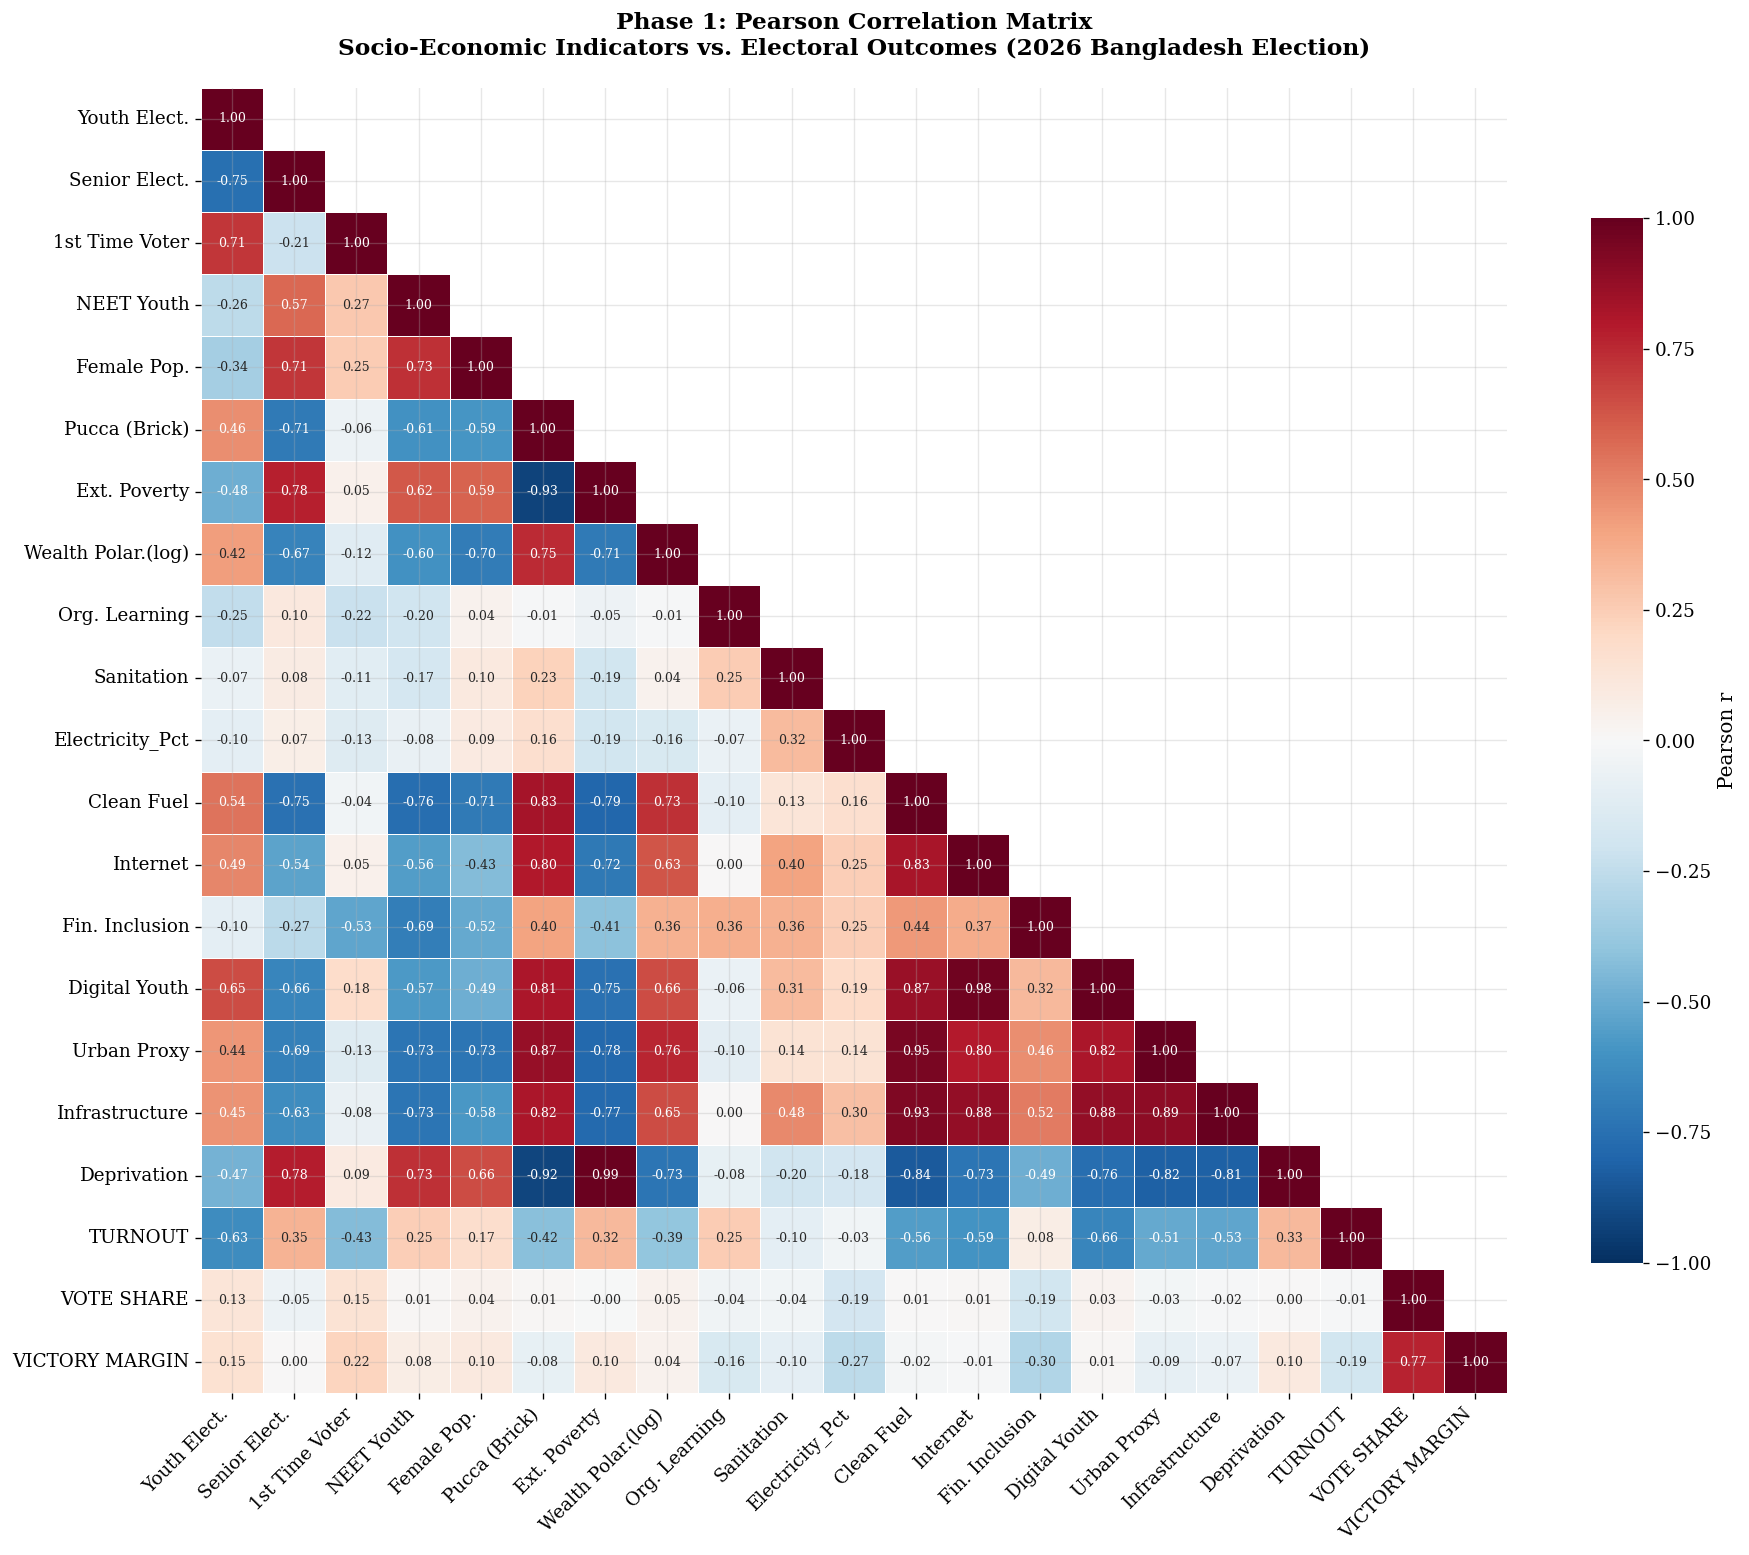
\includegraphics[width=\columnwidth]{exported_plots/Election_Visualization_Correlation_Heatmap.png}
\caption{Pearson correlation heatmap with electoral outcome variables positioned at bottom-right ($N = 268$).}
\label{fig:corr_heatmap}
\end{figure}

% ============================================================================
% VI. CLUSTERING ANALYSIS
% ============================================================================
\section{K-Means Clustering Analysis}

K-Means clustering was applied to discover latent socio-economic archetypes, independent of electoral outcomes. All 12 features were standardized via \texttt{StandardScaler}. The Silhouette Score was computed for $K \in \{2, \ldots, 10\}$ using \texttt{ClusteringEvaluator}.

$K = 2$ achieved the highest Silhouette Score of \textbf{0.7078}, indicating exceptionally strong cluster separation. Table~\ref{tab:clusters} profiles the two archetypes.

\begin{table}[t]
\centering
\caption{K-Means Cluster Profiles ($K = 2$, Silhouette = 0.7078)}
\label{tab:clusters}
\footnotesize
\begin{tabular}{l r r}
\toprule
\textbf{Feature} & \textbf{Cluster 0} & \textbf{Cluster 1} \\
 & \textbf{($N=235$)} & \textbf{($N=34$)} \\
\midrule
Pucca\_Pct & 16.41\% & 63.53\% \\
Extreme\_Poverty\_Pct & 66.18\% & 15.82\% \\
Internet\_Pct & 26.04\% & 49.46\% \\
Clean\_Fuel\_Pct & 10.79\% & 77.75\% \\
Voter\_Turnout\_Pct & 61.79\% & 49.11\% \\
\bottomrule
\end{tabular}
\end{table}

Cluster~0 (``Rural/Deprived,'' 87.4\%) exhibits high poverty, low connectivity, and \emph{higher} turnout (61.79\%). Cluster~1 (``Urban/Affluent,'' 12.6\%) captures metropolitan constituencies with high wealth and \emph{lower} turnout (49.11\%)---a 12.68 percentage point gap.

\begin{figure}[t]
\centering
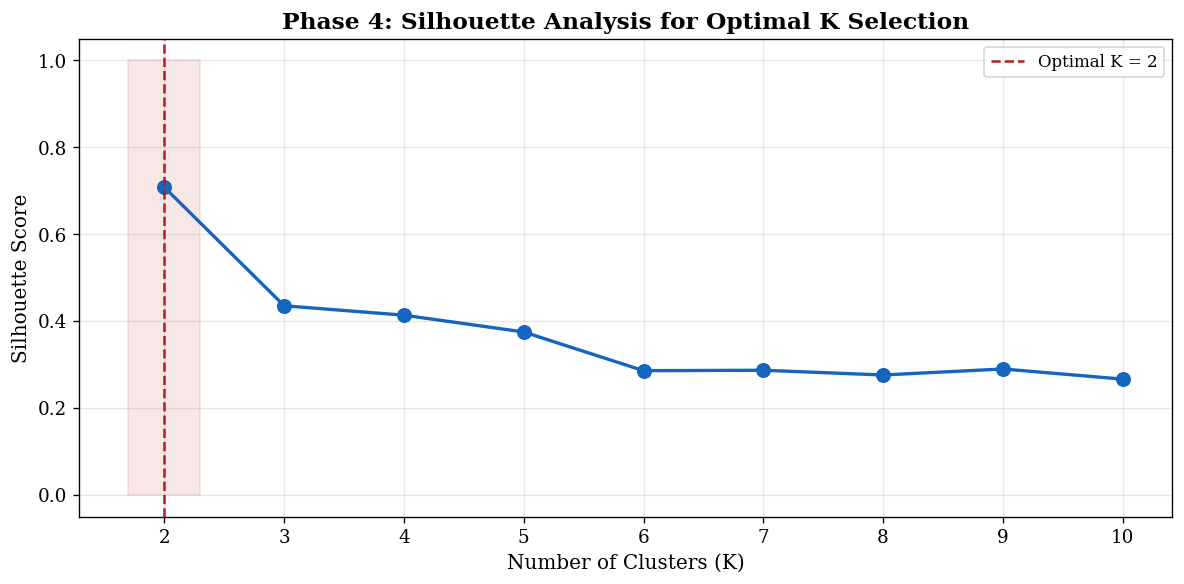
\includegraphics[width=\columnwidth]{exported_plots/Election_Silhouette_Score_Visualization.png}
\caption{Silhouette Score vs.\ $K$. Optimal $K = 2$ with Silhouette = 0.7078.}
\label{fig:silhouette}
\end{figure}

% ============================================================================
% VII. REGRESSION ANALYSIS
% ============================================================================
\section{Regression Analysis}

Two regression models were trained (Train: $N = 216$, Test: $N = 52$):

\textbf{Model A (Voter Turnout):} Linear Regression with ElasticNet regularization, combining L1 feature selection and L2 multicollinearity handling.

\textbf{Model B (Vote Share):} Random Forest Regressor for non-linear relationships.

\begin{table}[t]
\centering
\caption{Regression Performance ($N_{\text{test}} = 52$)}
\label{tab:regression}
\footnotesize
\begin{tabular}{l l r r r}
\toprule
& \textbf{Target} & \textbf{$R^2$} & \textbf{RMSE} & \textbf{MAE} \\
\midrule
A & Turnout & \textbf{0.6302} & 5.23\% & 4.44\% \\
B & Vote Share & $-0.0051$ & 9.54\% & 6.94\% \\
\bottomrule
\end{tabular}
\end{table}

Model~A achieves $R^2 = 0.6302$, explaining 63\% of turnout variance. The top predictors are Youth\_Electorate\_Pct (coeff = $-5.797$) and Senior\_Electorate\_Pct (coeff = $-5.777$), both negative---higher demographic concentration of either age extreme \emph{decreases} turnout. Model~B achieves $R^2 = -0.0051$, confirming that vote share is unpredictable from census data---it reflects campaign dynamics rather than structural conditions.

\begin{figure}[t]
\centering
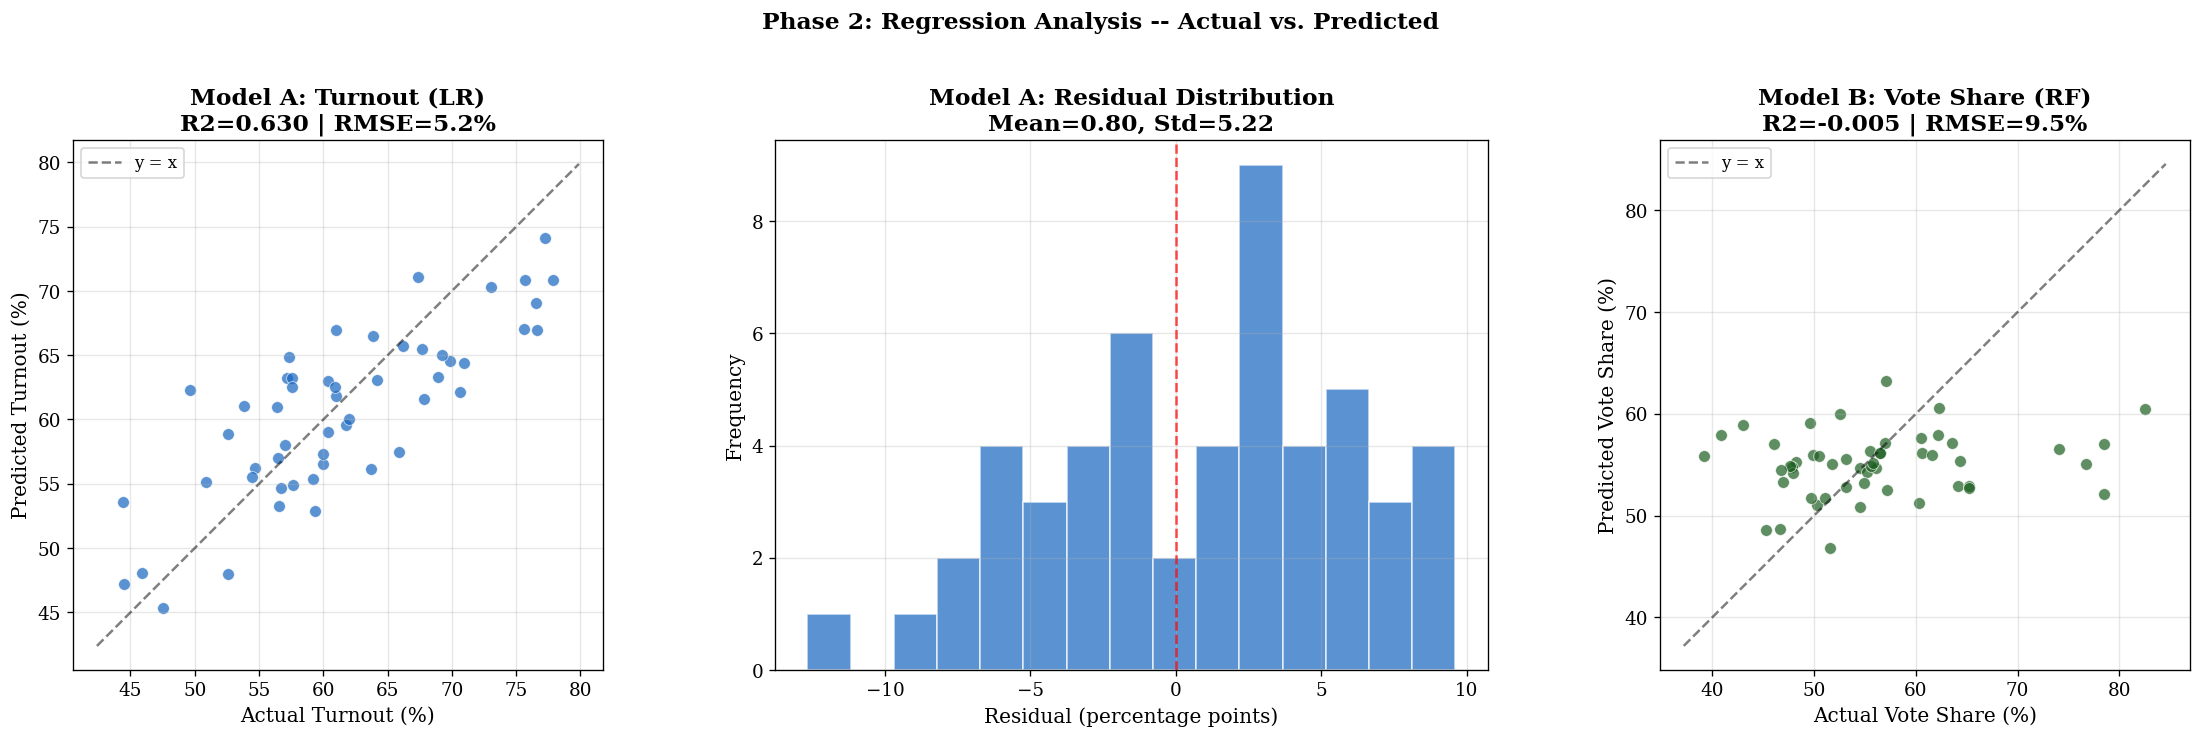
\includegraphics[width=\columnwidth]{exported_plots/Election_Visualizations_Actual_vs_Predicted_Plots.png}
\caption{Actual vs.\ Predicted plots: Model A (Turnout, $R^2 = 0.63$) and Model B (Vote Share, $R^2 \approx 0$).}
\label{fig:regression}
\end{figure}

% ============================================================================
% VIII. CLASSIFICATION MODEL
% ============================================================================
\section{Classification Model}

\subsection{Setup}
The capstone analysis predicts coalition victory (BNP vs.\ Jamaat/Reform) from census data. The minor INDEPENDENT\_OTHER class (6 seats) was excluded. Inverse-frequency class weighting was applied: $w_{\text{JAMAAT}} = 1.8264$, $w_{\text{BNP}} = 0.6885$. The K-Means \texttt{Cluster\_ID} was included as a feature. A stratified 80/20 split yielded Train: $N = 207$, Test: $N = 56$. A Random Forest Classifier with 200 trees was trained.

\subsection{Results}

\begin{table}[t]
\centering
\caption{Classification Performance ($N_{\text{test}} = 56$)}
\label{tab:classification}
\footnotesize
\begin{tabular}{l r | l r r r}
\toprule
\textbf{Metric} & \textbf{Value} & \textbf{Class} & \textbf{P} & \textbf{R} & \textbf{F1} \\
\midrule
Accuracy & 0.7679 & BNP & 0.81 & 0.87 & 0.84 \\
W-F1 & 0.7609 & Jamaat & 0.64 & 0.53 & 0.58 \\
AUC-ROC & 0.7738 & & & & \\
Baseline & 0.7262 & & & & \\
\bottomrule
\end{tabular}
\end{table}

The model surpasses the majority-class baseline by 4.16 percentage points. Fig.~\ref{fig:classification} shows the confusion matrix and feature importance ranking.

\subsection{Feature Importance}

The top features are Youth\_Electorate\_Pct (0.1259) and First\_Time\_Voter\_Pct (0.1201), together accounting for 24.61\% of discriminative power. The top~5 features cumulatively explain 44.05\% of Gini decrease. This establishes \textbf{youth demographics as the primary structural predictor of coalition victory}.

\begin{figure}[t]
\centering
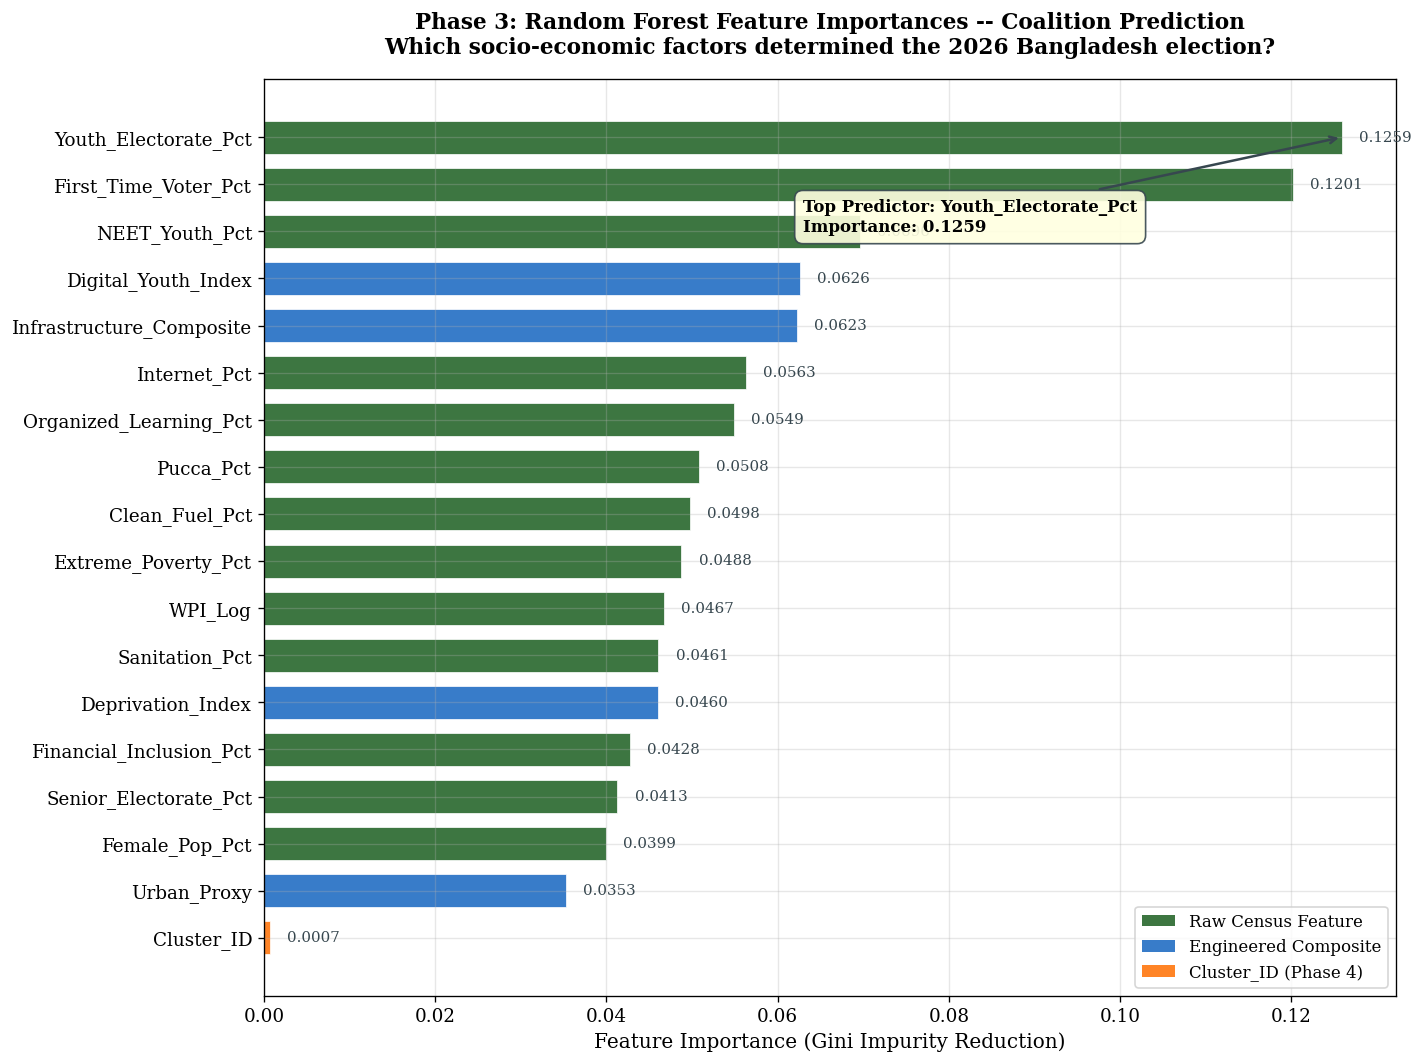
\includegraphics[width=\columnwidth]{exported_plots/Election_Visualization_Feature_Importance_Bar_Chart.png}
\caption{Feature importance ranking. Green: raw BBS features; Blue: engineered composites; Amber: K-Means Cluster\_ID.}
\label{fig:feat_imp}
\end{figure}

\begin{figure}[t]
\centering
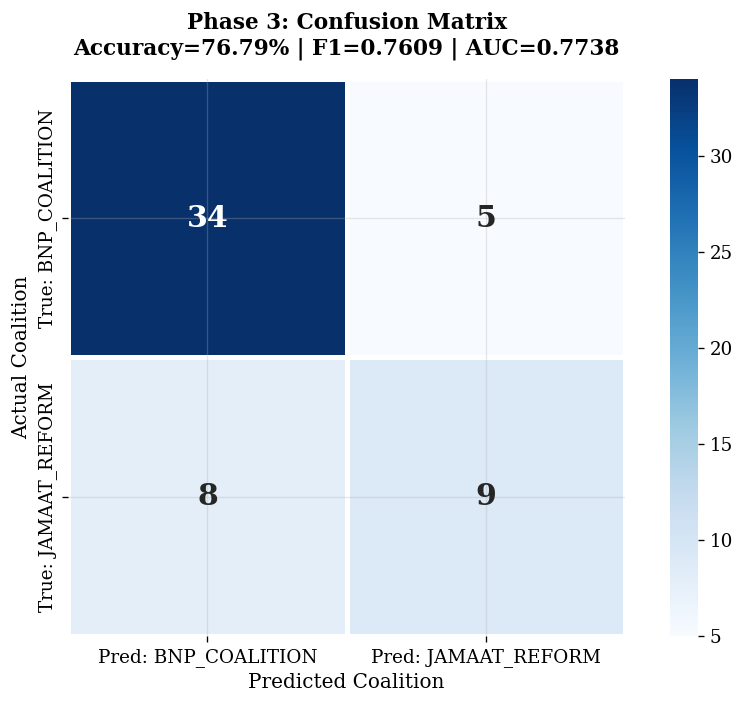
\includegraphics[width=0.75\columnwidth]{exported_plots/Election_Visualization_Confusion_Matrix.png}
\caption{Confusion matrix for Random Forest coalition classifier.}
\label{fig:classification}
\end{figure}

\subsection{Ablation Study}

Removing \texttt{Cluster\_ID} reduced accuracy from 0.7679 to 0.7500 ($\Delta = +0.0179$) and F1 from 0.7609 to 0.7453 ($\Delta = +0.0156$), confirming the unsupervised-to-supervised pipeline linkage provides genuine predictive value.

% ============================================================================
% IX. ADVANCED ANALYTICS
% ============================================================================
\section{Advanced Analytics Pipeline}

An extended pipeline was developed on the $N = 168$ constituency subset with referendum data.

\subsection{Extended Regression}
Referendum support prediction achieved $R^2 = 0.2836$ (RMSE = 7.9103), indicating that socio-economic features explain approximately 28\% of YES vote variance. Winning margin prediction yielded $R^2 = 0.0162$ (RMSE = 15.8063), confirming margin unpredictability.

\subsection{Extended Classification}
The referendum outcome classifier achieved \textbf{90.00\% accuracy} with AUC-ROC = \textbf{0.9136}, demonstrating that referendum outcomes are highly predictable via non-linear ensemble methods. Multi-class party prediction achieved 80.00\% accuracy (F1 = 0.7643), and voter behavior archetype classification achieved 80.00\% across 4 categories.

\begin{figure}[t]
\centering
\begin{subfigure}[b]{0.48\columnwidth}
    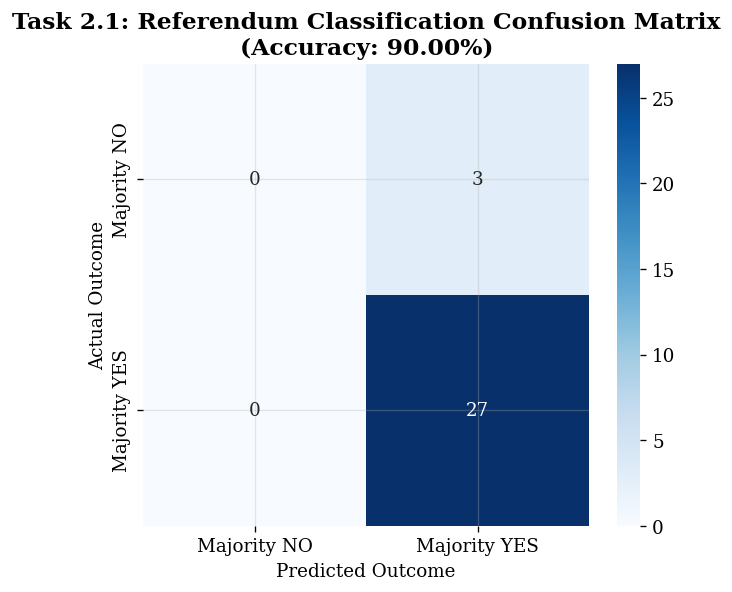
\includegraphics[width=\textwidth]{exported_plots/Advanced_1_Referendum_Outcome_Classification.png}
    \caption{Referendum (Acc = 0.90)}
\end{subfigure}
\hfill
\begin{subfigure}[b]{0.48\columnwidth}
    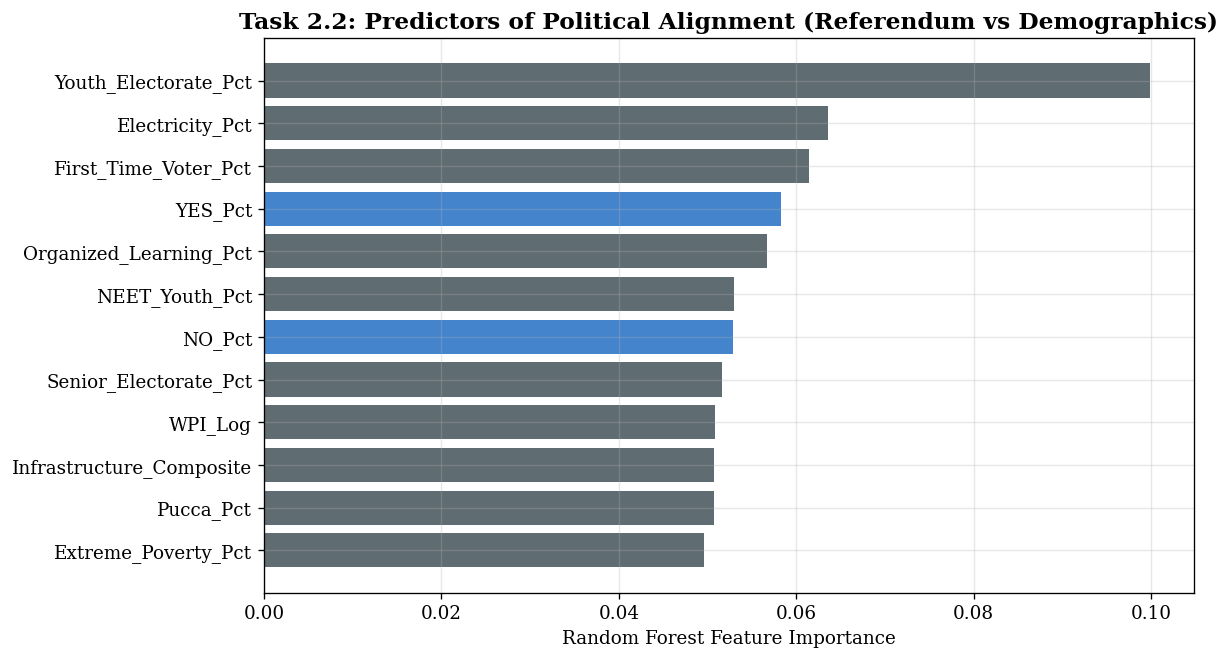
\includegraphics[width=\textwidth]{exported_plots/Advanced_2_Winning_Party_Prediction.png}
    \caption{Party (Acc = 0.80)}
\end{subfigure}
\caption{Extended classification confusion matrices.}
\label{fig:adv_class}
\end{figure}

\subsection{Political Alignment Clustering}
K-Means with $K = 4$ on political outcome features (Silhouette = 0.3776) identified four political tribes: anti-reform strongholds (NO = 62.94\%, high margin), pro-reform dominance seats (YES = 68.16\%), competitive high-turnout constituencies (margin = 12.18\%, turnout = 66.49\%), and competitive low-turnout urban seats.

% ============================================================================
% X. HYPOTHESIS TESTING
% ============================================================================
\section{Deductive and Advanced Hypothesis Testing}

Thirteen hypotheses were tested using quintile analysis, t-tests, correlation, feature importance, and logistic regression. Table~\ref{tab:hypotheses} summarizes the ten deductive hypotheses.

\begin{table}[t]
\centering
\caption{Deductive Hypothesis Testing Summary}
\label{tab:hypotheses}
\footnotesize
\begin{tabular}{c p{4.2cm} l}
\toprule
\textbf{H\#} & \textbf{Hypothesis} & \textbf{Verdict} \\
\midrule
1 & Elite/Wealth Reversal (U-shaped) & \textbf{Confirmed} \\
2 & Senior Citizen Firewall & Rejected \\
3 & Student/Youth Vanguard & Partial \\
4 & Referendum Generational Chasm & Rejected \\
5 & Gender Partisan Divide & Partial \\
6 & Digital Battleground & Rejected \\
7 & Border Radicalization & \textbf{Confirmed} \\
8 & Coalition Referendum Cleavage & \textbf{Confirmed} \\
9 & Digital Referendum Paradox & Weak \\
10 & Poverty Anti-Reform Backlash & Weak \\
\bottomrule
\end{tabular}
\end{table}

\subsection{H1: The Elite/Wealth Reversal}
Jamaat win rates by Pucca\_Pct quintile: Q1 = 37.74\%, Q2 = 21.15\%, Q3 = 15.09\%, Q4 = 25.00\%, Q5 = 37.74\%. The identical rates at Q1 and Q5 confirm a U-shaped ``horseshoe'' pattern---Jamaat draws support from both the poorest and wealthiest constituencies.

\begin{figure}[t]
\centering
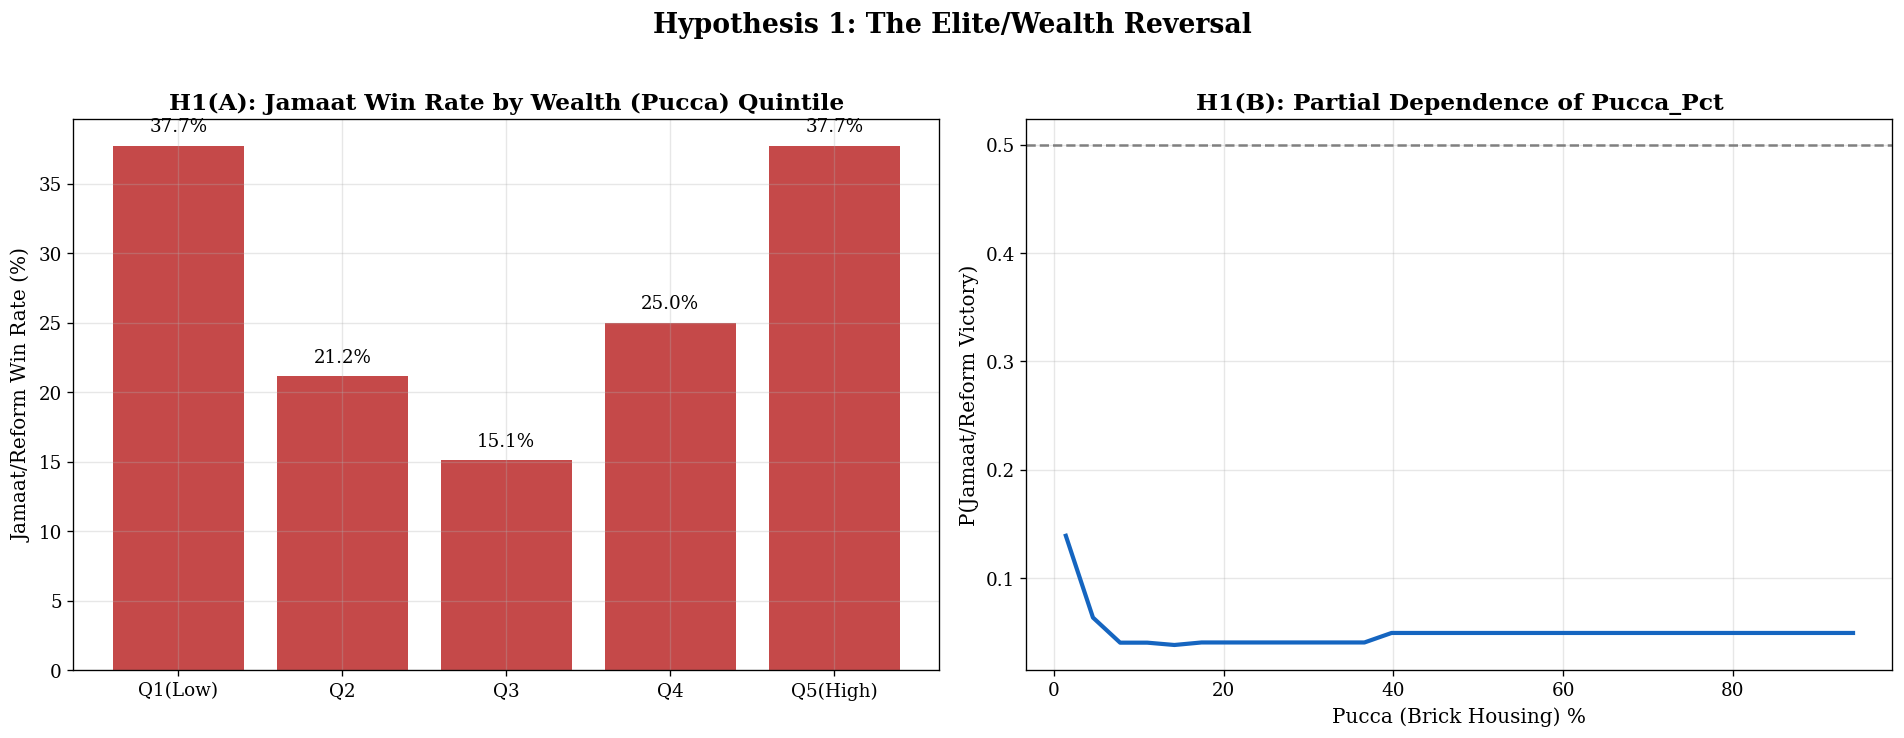
\includegraphics[width=\columnwidth]{exported_plots/Phase5_The_Elite_Wealth_Reversal.png}
\caption{H1: U-shaped Jamaat win rate by wealth quintile.}
\label{fig:h1}
\end{figure}

\subsection{H2: Senior Citizen Firewall}
BNP mean senior percentage: 13.22\%; Jamaat: 13.77\%. $t = -1.5284$, $p = 0.1289$---not significant. \textbf{Rejected.}

\subsection{H3--H6: Youth, Generational, Gender, Digital}
Student Vanguard Index importance = 0.0659 (H3, partial). Referendum generational correlations negligible: Senior vs.\ NO $r = 0.0062$, Youth vs.\ YES $r = -0.0341$ (H4, rejected). Female\_Pop\_Pct importance = 0.0469 (H5, partial). Internet\_Pct importance controlling for turnout = 0.0117 (H6, rejected).

\begin{figure}[t]
\centering
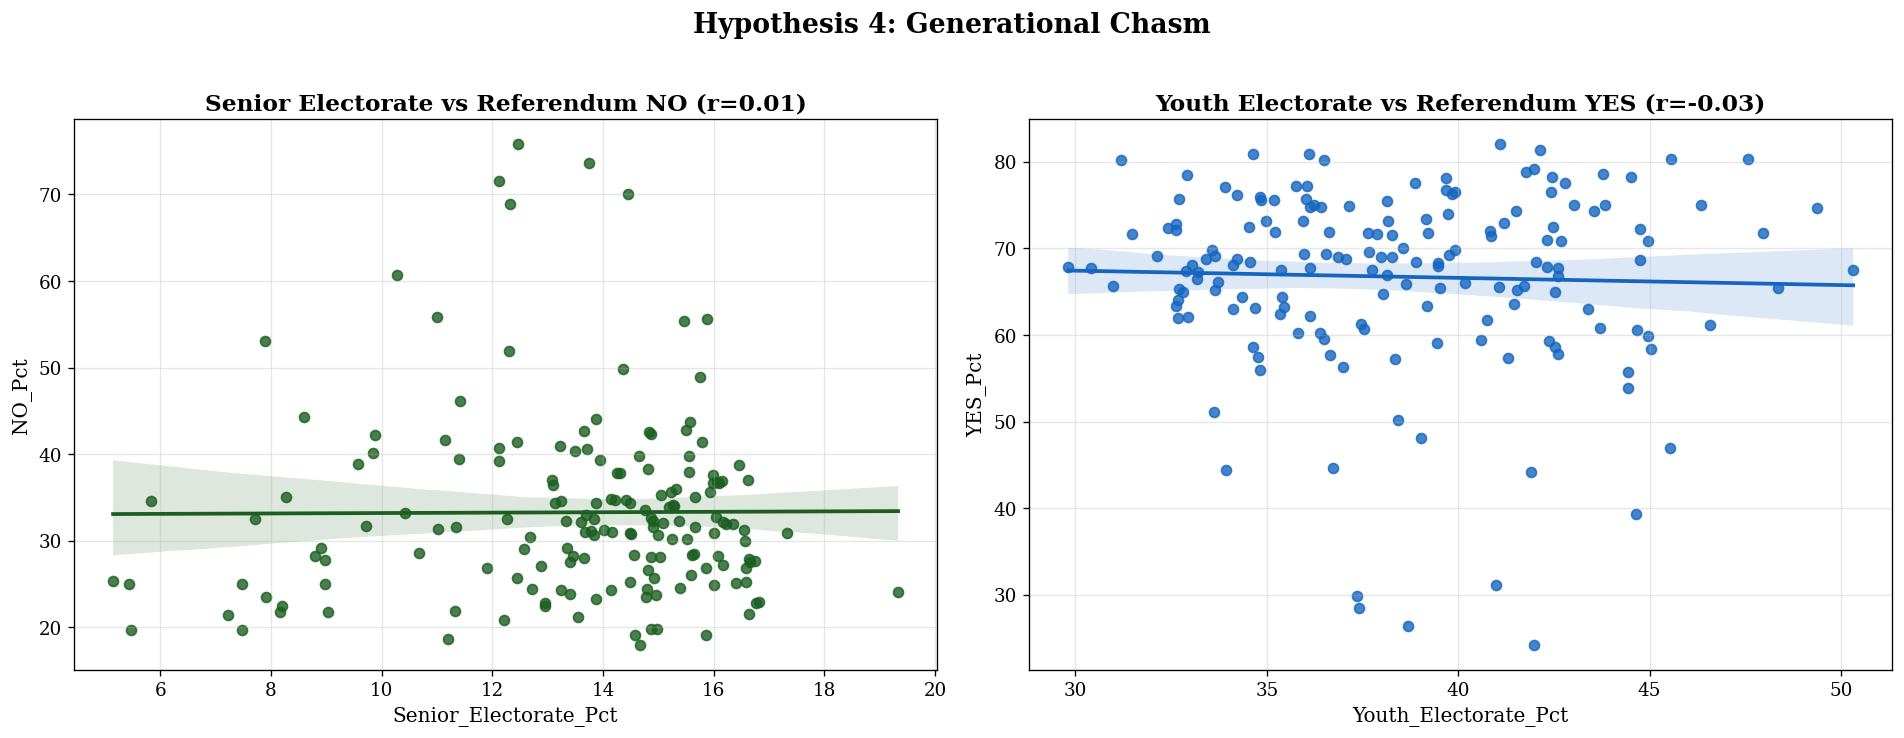
\includegraphics[width=\columnwidth]{exported_plots/Phase5_The_Referendum_Generational_Chasm.png}
\caption{H4: Referendum outcomes by age-structure. No generational chasm detected.}
\label{fig:h4}
\end{figure}

\subsection{H7: Border Radicalization}
Border Jamaat win rate: \textbf{34.1\%} vs.\ interior: 21.4\%. Odds ratio = \textbf{1.90}. Border constituencies are nearly twice as likely to elect Jamaat candidates. \textbf{Confirmed.}

\subsection{H8: Coalition Referendum Cleavage}
BNP mean NO\_Pct: \textbf{34.62\%}; Jamaat: 29.44\%. $p = 0.000781$---highly significant at $\alpha = 0.001$. \textbf{Confirmed.}

\begin{figure}[t]
\centering
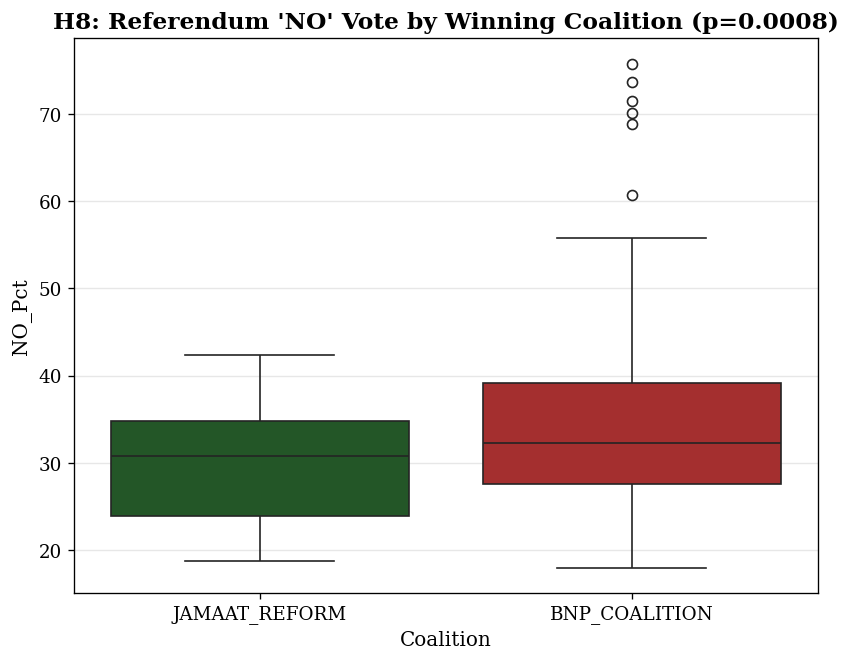
\includegraphics[width=\columnwidth]{exported_plots/Phase5_The_Coalition_Referendum_Cleavage.png}
\caption{H8: Referendum NO vote by coalition ($p = 0.000781$).}
\label{fig:h8}
\end{figure}

\subsection{H9--H10: Digital Referendum and Poverty Backlash}
Internet vs.\ YES: $r = 0.0952$ (H9, weak). Poverty vs.\ NO: $r = 0.0816$ (H10, weak). Both directions are consistent with hypotheses but magnitudes are insufficient for confirmation.

\subsection{Advanced Controversial Hypotheses}

\textbf{Hypothesis A (Horseshoe Wealth):} Decile-level analysis confirms the U-shaped Jamaat pattern at higher resolution.

\textbf{Hypothesis B (Digital Elitism):} Regression coefficient for unconnected youth predicting NO vote: $\beta = +0.3479$. Digitally excluded youth lean toward referendum rejection.

\textbf{Hypothesis C (Geopolitical Securitization):} Logistic coefficients: Extreme Poverty = $-0.0052$ (negligible), Border Proximity = $+0.6752$. Border effects on Jamaat support are \emph{independent} of poverty.

\begin{figure}[t]
\centering
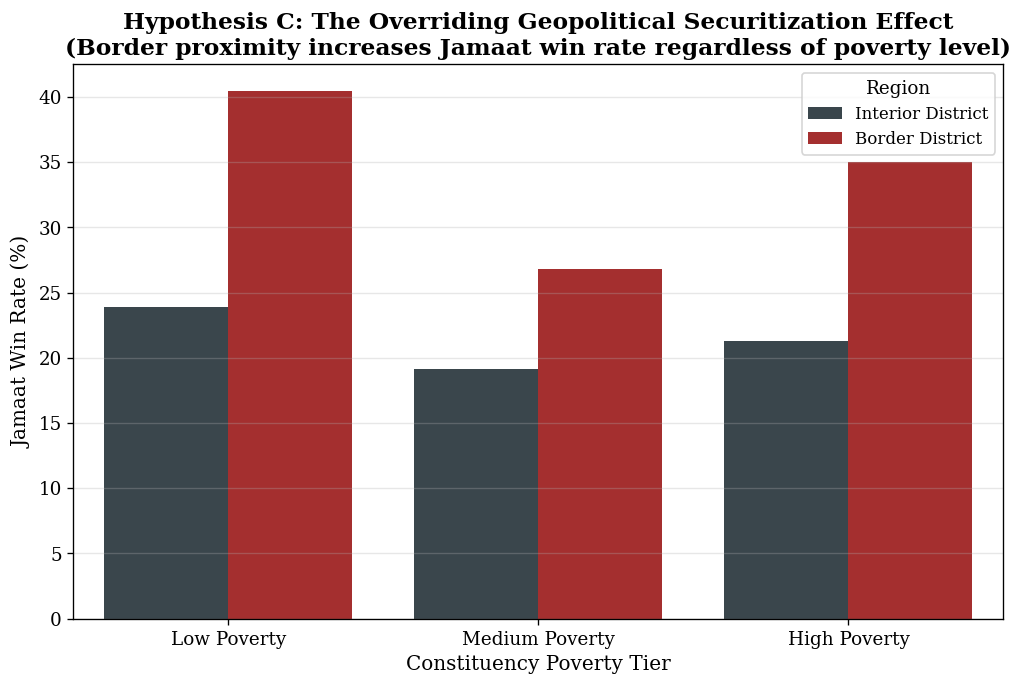
\includegraphics[width=\columnwidth]{exported_plots/Controversial_C_The_Geopolitical_Securitization_Effect.png}
\caption{Hypothesis C: Border proximity ($\beta = +0.6752$) drives Jamaat support independently of poverty ($\beta = -0.0052$).}
\label{fig:hyp_c}
\end{figure}

% ============================================================================
% XI. DISCUSSION
% ============================================================================
\section{Results and Discussion}

The pipeline yields six principal findings:

\begin{enumerate}
    \item \textbf{Youth as Primary Determinant:} Youth\_Electorate\_Pct (0.1259) and First\_Time\_Voter\_Pct (0.1201) together account for 24.61\% of classifier discriminative power.

    \item \textbf{Internet--Turnout Paradox:} Internet penetration shows the strongest correlation with turnout ($r = -0.5948$) but minimal coalition predictive power (importance = 0.0563)---it affects \emph{whether} people vote, not \emph{whom}.

    \item \textbf{Turnout Predictability vs.\ Margin Unpredictability:} Turnout $R^2 = 0.6302$; vote share $R^2 = -0.0051$. Participation is structurally determined; mandate strength is campaign-dependent.

    \item \textbf{U-Shaped Wealth Effect:} Both Q1 and Q5 favor Jamaat at 37.74\%, while Q3 favors BNP (Jamaat = 15.09\%).

    \item \textbf{Border Radicalization:} OR = 1.90, independent of poverty ($\beta_{\text{border}} = +0.6752$ vs.\ $\beta_{\text{poverty}} = -0.0052$).

    \item \textbf{Coalition--Referendum Cleavage:} The only statistically confirmed partisan divide on the referendum ($p = 0.000781$).
\end{enumerate}

The data reveals a deeply bifurcated electorate: 87.4\% rural-deprived constituencies with high turnout versus 12.6\% urban-affluent constituencies with low engagement. Coalition allegiance is primarily determined by generational composition---not wealth, gender, or digital access.

% ============================================================================
% XII. CHALLENGES AND LIMITATIONS
% ============================================================================
\section{Challenges and Limitations}

\textbf{Data Incompleteness:} Twelve districts lacked SDG census sheets, requiring KNN imputation. The July Charter referendum data was only confirmed for 168 of 300 constituencies at the time of analysis, limiting the generalizability of referendum-specific findings.

\textbf{Geospatial Approximation:} The BBS administrative hierarchy and Election Commission boundaries do not align perfectly. The ``majority proxy'' NLP mapping approach achieved 89.6\% coverage (269 seats), but excluded 31 constituencies, potentially introducing localized selection bias.

\textbf{Ecological Inference:} All analyses operate at the constituency aggregate level. Correlations do not strictly imply individual-level causal voting behavior.

% ============================================================================
% XIII. CONCLUSION
% ============================================================================
\section{Conclusion}

This paper presents a robust PySpark data pipeline analyzing the 2026 Bangladesh National Election. We successfully integrated heterogenous BBS census data with EC results across 269 constituencies. 

Our findings demonstrate that electoral participation (turnout) is structurally predictable from census data ($R^2 = 0.6302$), primarily driven by the absence of extreme demographic concentrations and an internet-turnout paradox ($r = -0.5948$). Conversely, vote share is unpredictable from demographics ($R^2 = -0.0051$). 

The Random Forest coalition classifier establishes youth demographics as the dominant predictor of partisan victory (Acc = 76.79\%, AUC = 0.7738). K-Means clustering highlights a severe urban-rural divide. Hypothesis testing confirms a U-shaped Elite/Wealth reversal for Jamaat support, significant border radicalization (OR = 1.90), and a notable coalition cleavage on the July Charter referendum ($p = 0.000781$).

Future work will expand this pipeline to incorporate 2018 and 2024 historical elections, assessing the temporal stability of these socio-economic determinants, and explore GIS-based polygon intersection to improve geospatial boundary mapping to 100\% coverage.

% ============================================================================
% REFERENCES
% ============================================================================
\balance
\begin{thebibliography}{99}

\bibitem{bbs2022}
Bangladesh Bureau of Statistics, ``Population and Housing Census 2022: National Report,'' Ministry of Planning, Government of the People's Republic of Bangladesh, 2023.

\bibitem{ec2026}
Bangladesh Election Commission, ``Results of the 13th National Parliamentary Election, February 12, 2026,'' Official Results Portal, 2026. [Online]. Available: \url{https://www.ecs.gov.bd}

\bibitem{spark}
M. Zaharia \emph{et al.}, ``Apache Spark: A Unified Engine for Big Data Processing,'' \textit{Commun. ACM}, vol. 59, no. 11, pp. 56--65, 2016.

\bibitem{mllib}
X. Meng \emph{et al.}, ``MLlib: Machine Learning in Apache Spark,'' \textit{J. Mach. Learn. Res.}, vol. 17, no. 34, pp. 1--7, 2016.

\bibitem{knn_impute}
O. Troyanskaya \emph{et al.}, ``Missing value estimation methods for DNA microarrays,'' \textit{Bioinformatics}, vol. 17, no. 6, pp. 520--525, 2001.

\bibitem{sklearn}
F. Pedregosa \emph{et al.}, ``Scikit-learn: Machine Learning in Python,'' \textit{J. Mach. Learn. Res.}, vol. 12, pp. 2825--2830, 2011.

\end{thebibliography}

\end{document}
